%% ==============
\section{Modellgetriebene Generierung von Dokumentation}
\label{ch:sec:}
%% ==============

%% ==============
\subsection{Topcased Gendoc}
\label{ch:sec:}
%% ==============

% Modellierung standardisiert OMG MDA, graduelle verfeinerung
% Anstrengungen der MDA si
% MDSD an diesem Beispiel kurz erkl�ren

Ein weiteres Werkzeug zur automatischen Generierung von Dokumentation ist das
in der Topcased Plattform enthaltene Gendoc, das aus Quellmodellen modellgetriebene
Erstellung von Dokumentation erm�glicht. Die Model Driven Architecture (MDA),
ein Standard zur modellgetriebenen Entwicklung der OMG\cite{Miller2001}, sieht
eine Unterteilung in mehreren Modellebenen unterschiedlicher Abstraktion vor.
Beginnend mit einem Modell der Dom�ne werden durch graduelle Verfeinerungen
Details zur Bearbeitung von Informationen bis hin zu der Spezifizierung der
konkreten technischen Implementierung, um aus den Modellen das fertige System zu
generieren.
% ============================================= %
Topcased\footnote{http://www.topcased.org/ ab 2014 auf http://polarsys.org/} ist
ein Open-Source Werkzeug f�r modellgetriebene Entwicklung und dient dem System-
und Software-Engineering von kritischen und embedded Anwendungen
\cite{Pontisso06}. Die Plattform unterst�tzt alle Entwicklungsstufen von der
Anforderungsanalyse bis zu der Implementierung. Sie basiert auf der Eclipse
Plattform und benutzt das Eclipse Modeling Framework (EMF), um einen
modellgetriebenen Arbeitsfluss zu realisieren. Es unterst�tzt neben UML Modellen
auch andere von der OMG standardisierten Modellierungssprachen wie
SysML\footnote{http://www.sysml.org/} und
ReqIF\footnote{http://www.omg.org/spec/ReqIF/}.
% ============================================= %
Als Teil der Topcased Plattform erlaubt Gendoc die Generierung von textueller
Dokumentation aus UML Modellen. Die Generierung wird von Skripten in den
Dokumenten-Templates, die Logik und Modellabfragen beinhalten, gesteuert. Um die
Modellabfrage zu realisieren sind
Acceleo\footnote{http://www.eclipse.org/acceleo/} Skripte und Object Constraint
Language (OCL)\footnote{http://www.omg.org/spec/OCL/} Ausdr�cke m�glich.

%% ==============
\subsection{Gendoc Realisierung}
\label{ch:sec:}
%% ==============

Acceleo Skripte, die direkt in den Dokumenten-Templates geschrieben werden lesen
die Quellmodelle mit Hilfe von OCL aus und f�llen das Dokument.
Die benutzten Skripte, die in der Acceleo Sprache geschrieben sind, k�nnen
beliebig Komplexe OCL Ausdr�cke wie Schleifen oder Logik enthalten. Die Skripte
sind in einer Markup-�hnlichen Sprache eingebettet, die HTML �hnliche
Unterst�tzung von Bildern und Listen besitzen.\\
% ============================================= %
Topcased unterst�tzt einen Gro�teil der UML Modelle, namentlich sind das
Klassen-, Komponenten- und Deployment-Diagrammes, die die Struktur beschreiben
und Sequenz-, Aktivit�ts- und Zustandsdiagramme die die dynamischen Teile eines
Systems beschreiben. Auch Use-Case Diagramme k�nnen modelliert, abgefragen und
in die Dokumentation mit eingebunden werden.\\
% ============================================= %
Der generative Ansatz verl�uft wie in Abbildung \ref{fig:topcased-gendocflow}
dargestellt. Die Modelle und die Dokumenten-Templates sind die Eingaben des
Systems, als Ausgabe liefert Gendoc das ausgef�llte Dokumenten-Template. Die
Abspeicherung der ODT\footnote{Open Document Text} und DOCX\footnote{Microsoft
Word Dokumenten Format} Formate als XML, erlaubt es Gendoc die Skripte zu
extrahieren und Auszuwerten. Da die Skripte in der Modelltransformationssprache
Acceleo geschrieben sind k�nnen sie direkt auf die Modelle ausgef�hrt werden.
Dieser Ansatz erlaubt es, alle von der EMF unterst�tzten Modellformate in Gendoc
einzusetzen. Gendoc erlaubt es auch im Batch-Modus zu laufen, um automatisierte
Werkzeugketten zu realisieren.\\
% ============================================= %
Beim Auswerten der Skripte behalten die Ausgaben die Formatierung bei. Dies
bedeutet aber auch, dass der Quell-Code im Template-Dokument unterschiedliche,
f�r Code untypische, Formatierungen besitzt, was das bearbeiten erschwert. Da
aber die Formatierung des Dokuments beibehalten wird ist die dynamische
Verlinkung mithilfe der Dokumenteneigenen Mechanismen m�glich. Graphische
Elemente, wie konkrete Diagramme k�nnen aus dem Quellmodell generiert werden und
neben dem Text in das generierte Dokument eingef�gt werden.

\begin{figure}[htp]
\begin{center}
  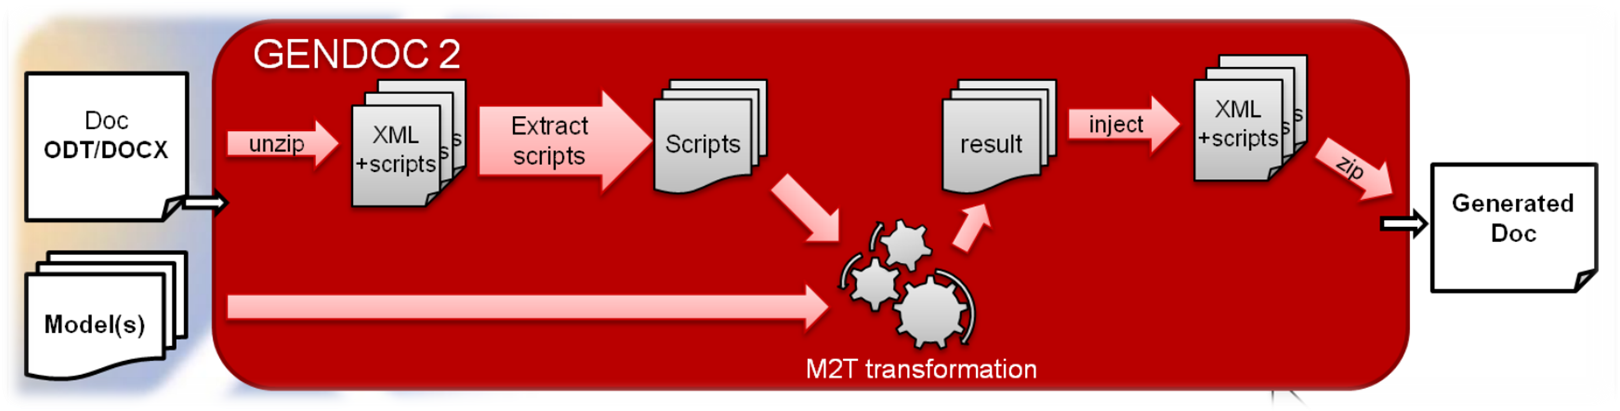
\includegraphics[width=1\textwidth]{img/topcased-gendocflow.png}
  \caption[Architektur des Gendoc Werkzeugs]{Architektur des Gendoc Werkzeugs}
  \label{fig:topcased-gendocflow}
\end{center}
\end{figure}

% Gendoc Befehlen werden durch das <gendoc> tag gekennzeichnet. Neben dem Acceleo
% Skript sind auch statische Texte mit Formatierungen, Bilder und Tabellen
% Erlaubt.
% 
% Die Konfiguration, die die Erstellung des Dokumentes steuert wird auch im
% Dokument-Template unter einem Markup-Tag gespeichert.
% 
% Ein Mechanismus zur Wiederverwendung von Code in den Templates steht zur
% Verf�gung.
% 
% Zugriff auf alle Elemente der Diagramme die benutzt weredn um das System zu
% modellieren. Volle Kontrolle auf die Erstellung des Dokumentes und der
% Informationen die aus den Modellen abgeleitet werden.

% Nachteil: Code aus Templates kann nur mit gro�em Aufwand auf ein Anderes
% Template angewandt werden.

% 
% 
% Wie funktioniert es?
% 	Konzeptuell
% 	Technische realisierung

	
% Listing erkl�ren was die einzelnen tags machen. Are rost listingu? Vezi daca se
% merita la dopler.
% % =======
% \lstset{breaklines=true,language=XML,caption={Das Element
% \emph{doplerdocplaceholder} mit dem \emph{doplerdoc} Attribut dient als
% Platzhalter f�r den K�hlungsmechanismus \emph{cooling\_mech}
% \cite{Rabiser2010}},label=lst:dopler_docbook_xml}
% \lstinputlisting[language=XML]{listings/topcased.xml}
% % =======

